\documentclass{standalone}
\usepackage{tikz}
\usepackage{xcolor}
\usetikzlibrary{shapes.geometric, arrows, positioning, fit, backgrounds, arrows.meta, calc}

\tikzstyle{block} = [rectangle, rounded corners, 
minimum width=6cm, 
minimum height=3cm,
text centered, 
draw=black, 
fill=gray!30]

\begin{document}

\begin{tikzpicture}


\node (sc) [block] {SiteControl};
\node (bc) [block, below=4cm of sc,align=center] {Bargecontrol \\ cabinet};
\node (cbc) [block, below=4cm of bc,align=center] {Power distribution \\ cabinet};

\node (glam1) [right=5cm of bc,scale=0.5] {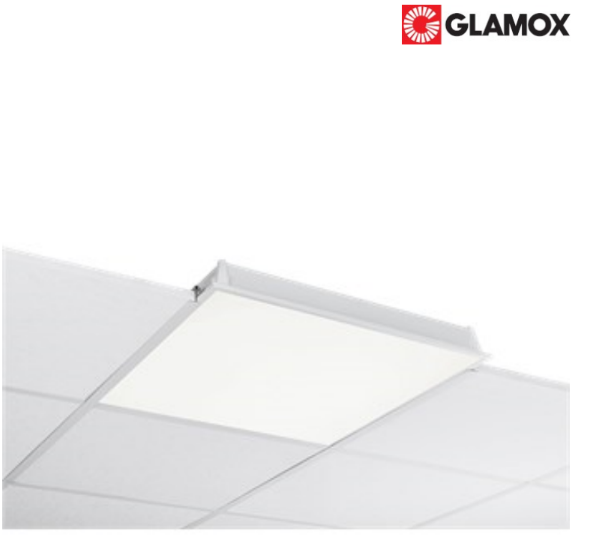
\includegraphics[width=\textwidth]{dali_glam1.png}};
\node (glam2) [right=5cm of glam1,scale=0.5] {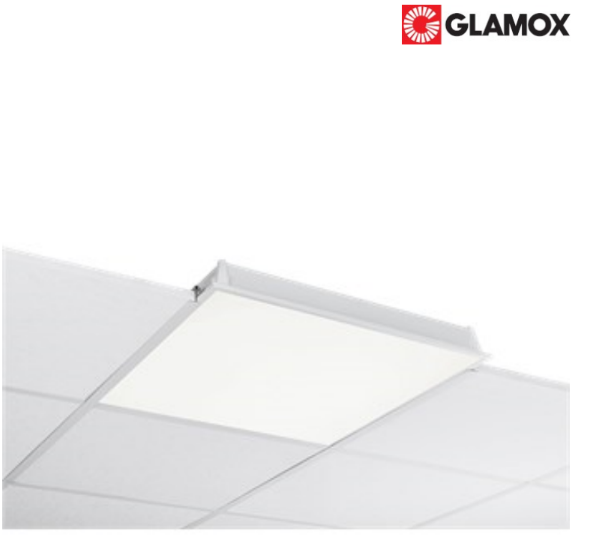
\includegraphics[width=\textwidth]{dali_glam1.png}};
\node (glam3) [right=5cm of glam2,scale=0.5] {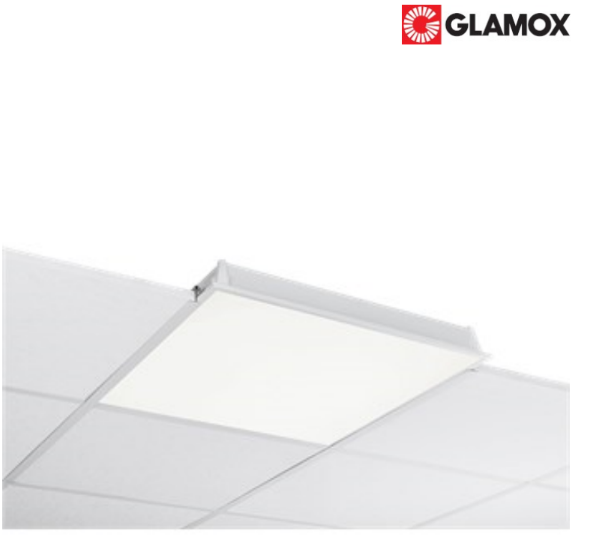
\includegraphics[width=\textwidth]{dali_glam1.png}};
\node (glam4) [right=5cm of glam3,scale=0.5] {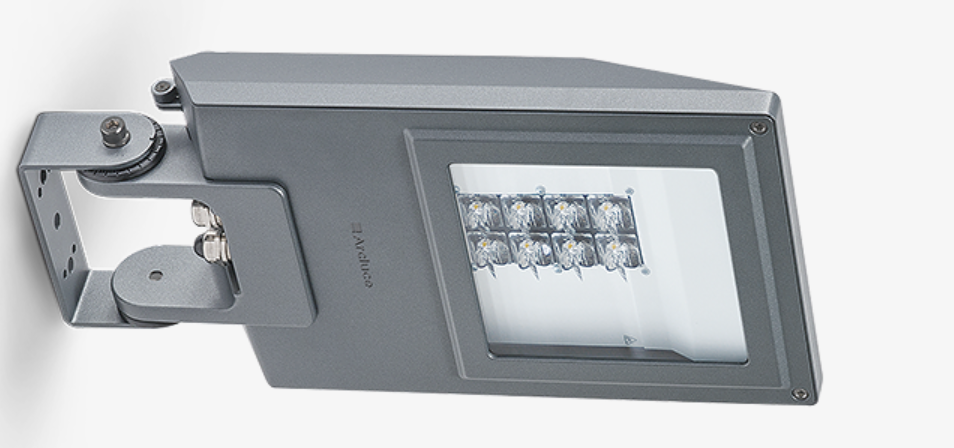
\includegraphics[width=\textwidth]{dali_glam2.png}};

\node (dali_switch) [below right=2cm and 0cm of glam1,scale=0.5] {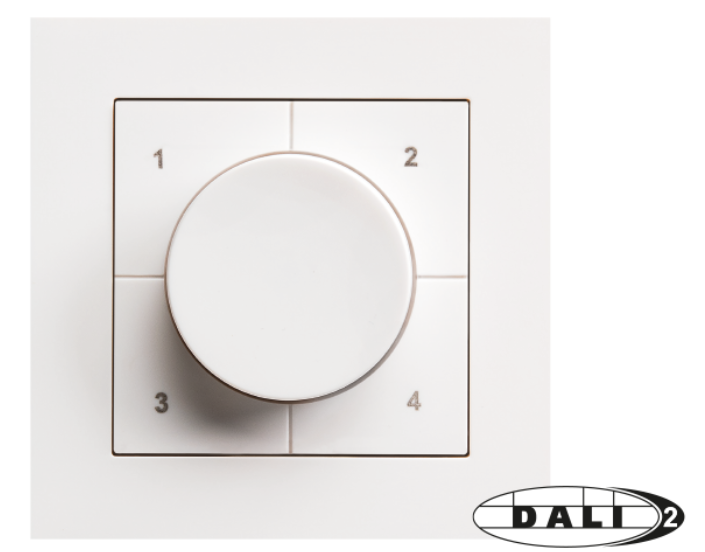
\includegraphics[width=\textwidth]{dali_switch.png}};
\node (dali_motion) [below right=2cm and 0cm of glam2,scale=0.5] {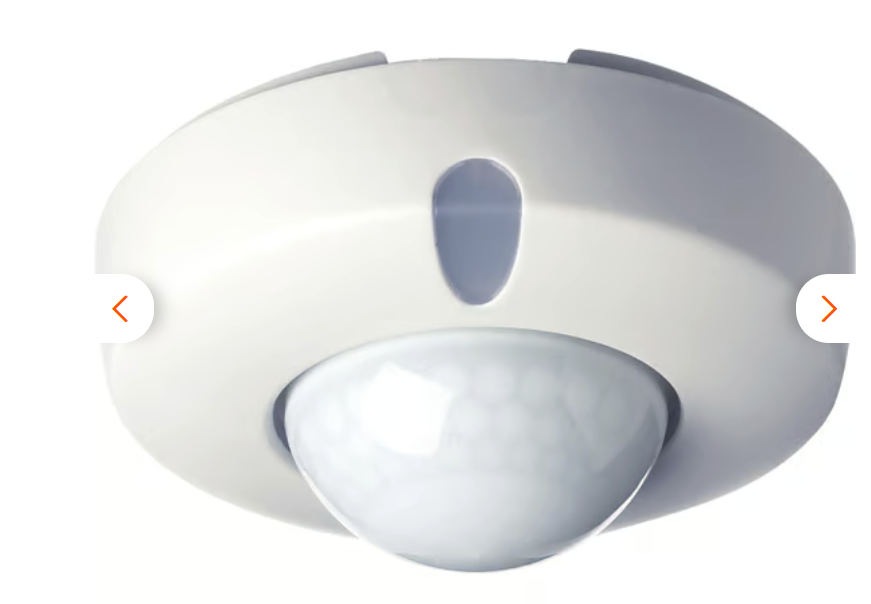
\includegraphics[width=\textwidth]{dali_motion.png}};

\node (thermostat) [right=5cm of glam4,scale=0.5] {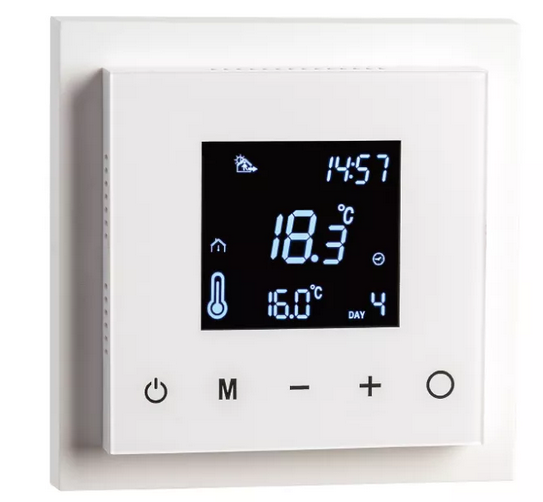
\includegraphics[width=\textwidth]{thermostat.png}};
\node (wifi) [above=1cm of thermostat,scale=0.2] {
\includegraphics[width=\textwidth]{mqtt-wifi.png}};
\node (heatpump) [right=3cm of thermostat,scale=1] {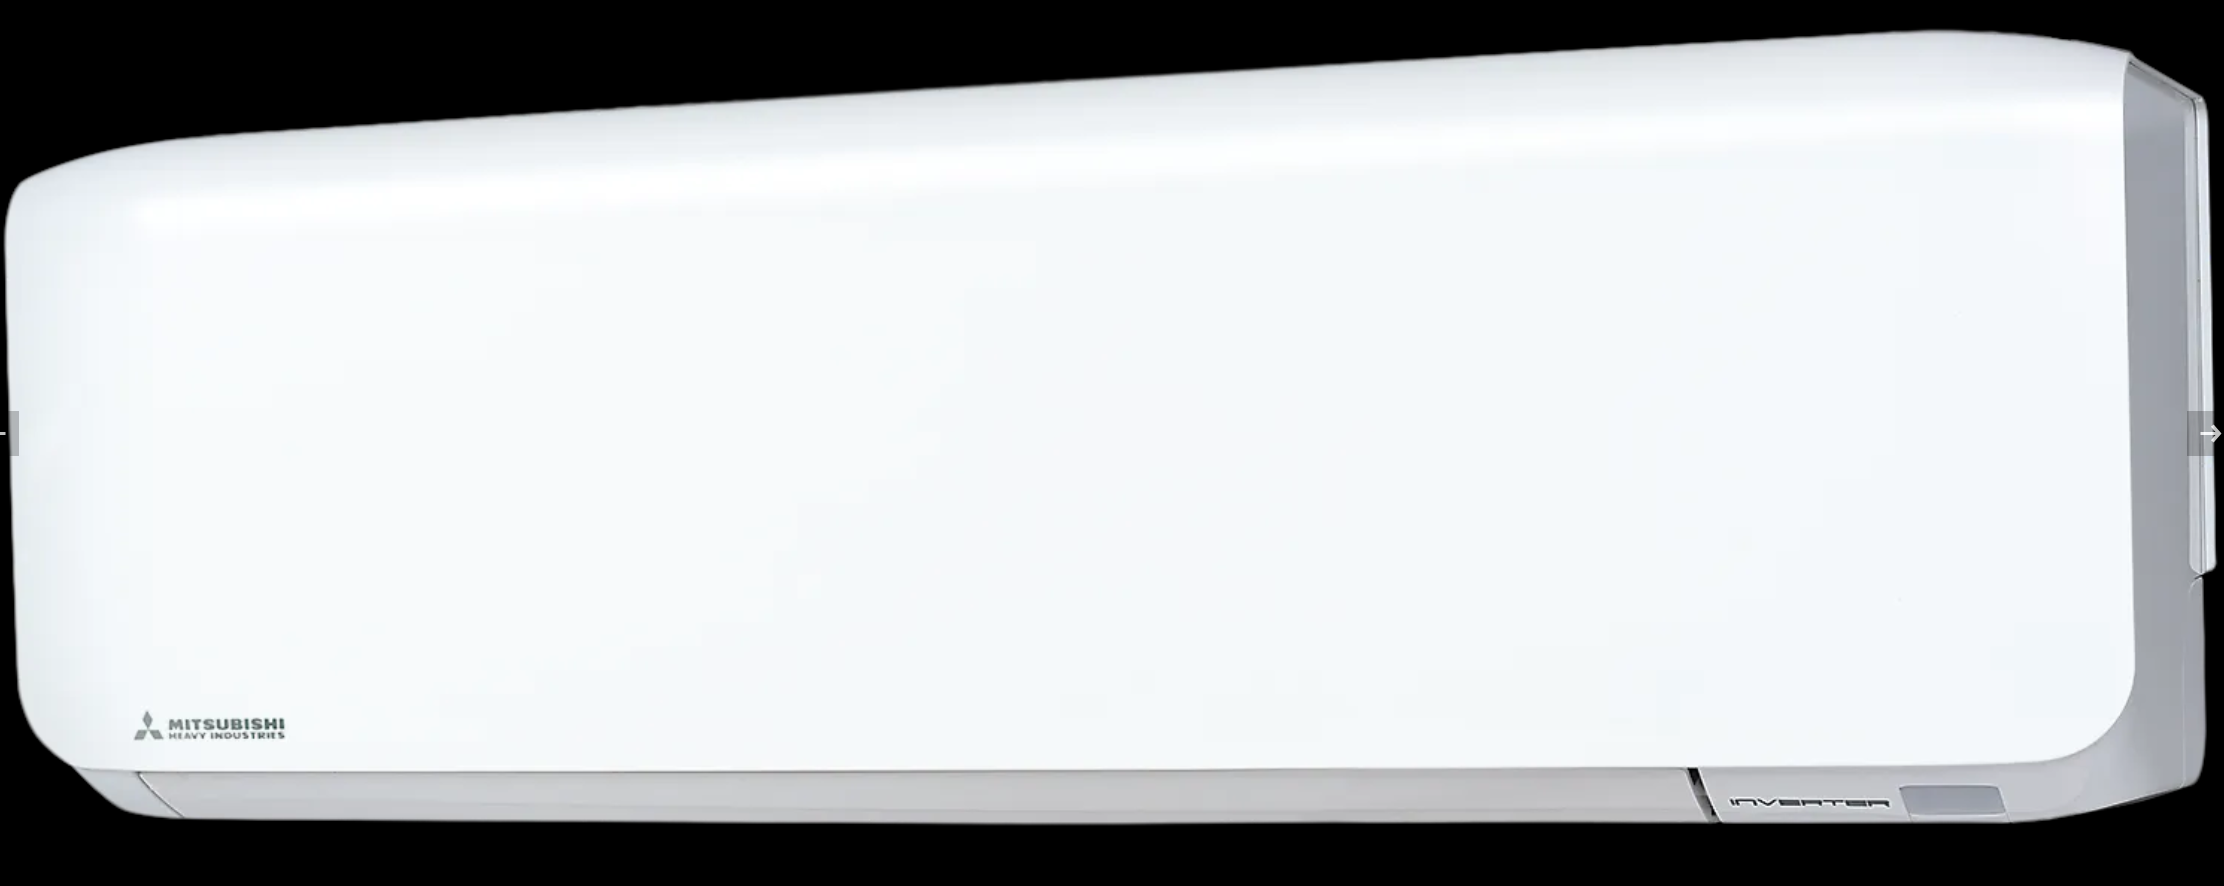
\includegraphics[width=\textwidth]{heat_pump_netsu.png}};
\node (modbus) [above=1cm of heatpump,scale=0.5] {
\includegraphics[width=\textwidth]{modbus.png}};


\draw [dashed,color=blue] (sc) -- (bc) node[midway,left] () {OPC UA};
\draw [dashed,color=green] (bc) -- (glam1) node[midway,above] () {DALI};
\draw [dashed,color=green] (glam1) -- (glam2) node[midway,above] () {DALI};
\draw [dashed,color=green] (glam2) -- (glam3) node[midway,above] () {DALI};
\draw [dashed,color=green] (glam3) -- (glam4) node[midway,above] () {DALI};
\draw [dashed,color=green] (dali_switch) |- (glam2);
\draw [dashed,color=green] (dali_motion) |- (glam3);

\draw [dashed,color=red] (cbc.east) -- +(2,0) node[midway,above] () {230VAC} |- ($(glam1.west)+(0,-1)$);
\draw [dashed,color=red] ($(glam1.east)+(0,-1)$) -- ($(glam2.west)+(0,-1)$) node[midway,above] () {230VAC};
\draw [dashed,color=red] ($(glam2.east)+(0,-1)$) -- ($(glam3.west)+(0,-1)$) node[midway,above] () {230VAC};
\draw [dashed,color=red] ($(glam3.east)+(0,-1)$) -- ($(glam4.west)+(0,-1)$) node[midway,above] () {230VAC};
\draw [dashed,color=red] ($(glam4.east)+(0,-1)$) -- ($(thermostat.west)+(0,-1)$) node[midway,above] () {230VAC};
\draw [dashed,color=red] ($(thermostat.east)+(0,-1)$) -- ($(heatpump.west)+(0,-1)$) node[midway,above] () {230VAC};

\draw [dashed,color=magenta] (wifi) |- +(-20,2) node[above] {MQTT over WiFi} -- (sc);
\draw [dashed,color=cyan] (modbus) |- ($(sc.east)+(0,1)$) node[midway,above,xshift=-32cm] () {Modbus TCP/IP};

\end{tikzpicture}



\end{document}